\section{Approccio Metodologico}

%\textit{This is the central and most important section of the report. Its objective must be to show, with linearity and clarity, the steps that have led to the definition of a decision model. The description of the working hypotheses, confirmed or denied, can be found in this section together with the description of the subsequent refining processes of the models. Comparisons between different models (e.g. heuristics vs. optimal models) in terms of quality of solutions, their explainability and execution times are welcome. }

%\textit{Do not attempt to describe all the code in the system, and do not include large pieces of code in this section, use pseudo-code where necessary. Complete source code should be provided separately (in Appendixes, as separated material or as a link to an on-line repo). Instead pick out and describe just the pieces of code which, for example:
%\begin{itemize}
%\item are especially critical to the operation of the system;
%\item you feel might be of particular interest to the reader for some reason;
%\item  illustrate a non-standard or innovative way of implementing an %algorithm, data
%structure, etc..
%\end{itemize}}

%\textit{You should also mention any unforeseen problems you encountered when implementing the system and how and to what extent you overcame them. Common problems are: difficulties involving existing software.} \\
 



Il dataset, ottenuto al termine della fase di analisi, risulta composto da 39 features rispetto alle 143 di partenza.
Viene quindi effettuata una fase di preprocessing allo scopo di ottenere una rappresentazione dei dati processabile efficacemente dalla rete neurale. Vengono tentati due approcci differenti: \textit{Factor Analysis of Mixed Data (FAMD)} \cite{famd} e  \textit{One Hot Encode (OHE)}. 
FAMD è un principal component method dedicato all'analisi di dataset contenenti variabili sia qualitative che quantitative, permettendo di analizzarne la similarità tra gli individui utilizzando variabili di diverso tipo.
Utilizzando i metodi implementati dalla libreria \texttt{prince} viene trasformato l'intero dataset (ad eccezione della variabile target), ottenendo il \textit{dataset FAMD}, composto da 38 features numeriche.
La libreria \texttt{OneHotEncoder} di \texttt{sklearn.preprocessing} ha invece permesso di codificare le features categoriche (non accettate dalle reti neurali) in binarie, ottenendo il \textit{dataset OHE}, composto da 113 colonne.
Per entrambi i dataset, viene eseguita una prima divisione (80-20) in training e test set e una seconda divisione del training in train e validation set (80-20). 
Dopodiché, le variabili target di ogni set sono state scalate nel range 0-3 e codificate con OHE e per il dataset OHE è stato utilizzato \texttt{StandardScaler()} per scalare i dati di train, validation e test, rendendoli comparabili fra loro.


\subsection{Reti neurali senza regolarizzazione}
Vengono eseguite sperimentazioni con i due dataset, per capire quale predica in modo migliore la classe target.
Per ottenere un'inizializzazione dei pesi non randomica è stato fissato un ramdom seed, \texttt{initializer = tf.keras. initializers.GlorotUniform(seed=1234)}, poi utilizzato in ogni modello. 


\subsubsection{Rete OHE}
Il metodo \texttt{NeuralNetwork()} viene definito per creare la rete neurale per il dataset OHE, in seguito citata come ``rete base". 
Si tratta di una rete (vedi Figura \ref{fig:neuralNetwork}) composta da 5 fully connected layer con un numero di neuroni decrescente (128, 64, 32, 16, 4), adatto a un numero alto di feature (113), e con funzione di attivazione \texttt{relu}. Questa specifica struttura della rete è stata scelta in seguito a numerosi tentativi in cui è stato modificato il numero di layer e il numero di neuroni.
Sono stati scelti \texttt{softmax} come funzione di attivazione dell'ultimo layer e \texttt{categorical\_crossentropy} come loss, in quanto opzioni più adatte per eseguire una classificazione su 4 classi. 
L'optimizer \texttt{adam}, invece, è stato scelto perché meglio performante di altri ottimizzatori testati e ha riportato i risultati migliori con il \textit{learning rate} di default. 
Viene inoltre tenuta traccia della metrica \textit{accuracy} per valutare le prestazioni del modello.
La rete base, come tutte le successive, è stata infine addestrata per 300 epoche, al fine di capirne meglio l'andamento su un numero di iterazioni sufficientemente lungo, e un \texttt{batch\_size} di 128, compromesso tra diverse dimensioni, nessuna particolarmente migliore delle altre.

\subsubsection{Rete FAMD}

Il metodo \texttt{NeuralNetwork\_famd()} viene invece definito per creare la rete neurale per il dataset FAMD. Si tratta di una rete composta da 4 fully connected layer con un numero di neuroni decrescente (64, 32, 16, 4), adatto a un numero di feature (38) non molto alto, ottenendo un modello con un numero decisamente minore di parametri. 
Per quanto riguarda tutti gli altri iperparametri sono stati mantenuti gli stessi usati nella rete base.
\begin{figure}[H]
     \centering
     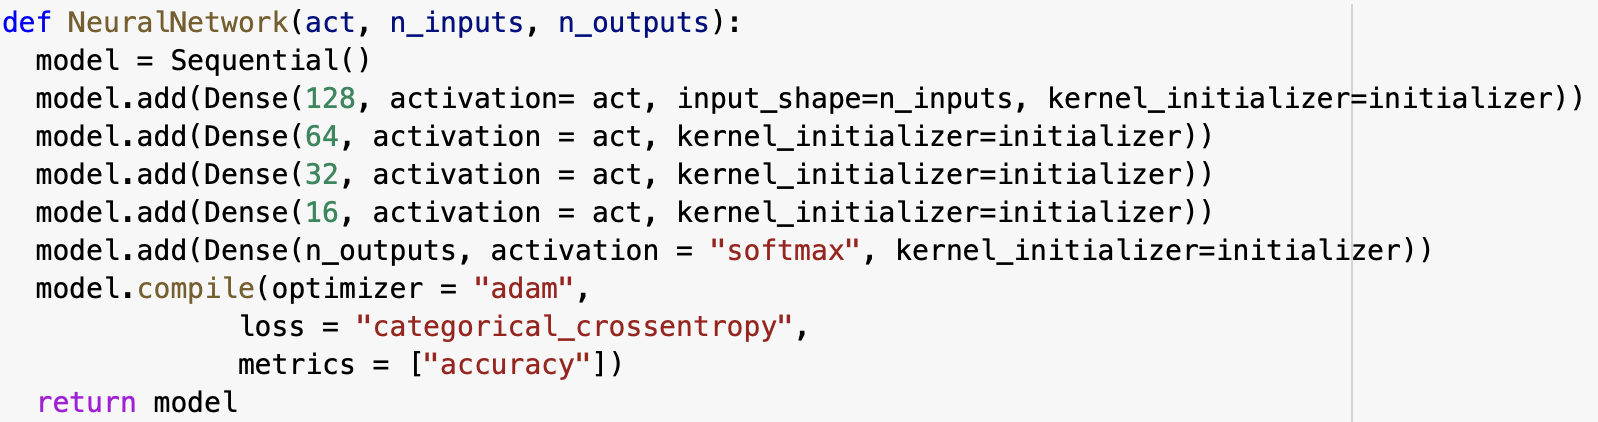
\includegraphics[scale=0.40]{Latex template for Project Report-20220108/immagini/NeuralNetwork.png}
     \caption{Codice metodo Neural Network}
     \label{fig:neuralNetwork}
\end{figure}
Dalle sperimentazioni, il dataset OHE risulta essere quello che
consente di ottenere i risultati migliori (vedi Figura \ref{fig:primiModelli}); motivo per cui verrà impiegato per tutti i successivi test. 
Per migliorare la rete base e contrastare il fenomeno dell'overfitting sono state utilizzate varie tecniche di regolarizzazione (\textit{Dropout}, \textit{L1}, \textit{L2} e \textit{Early Stopping}), mentre per sopperire allo sbilanciamento dei dati è stato usato \textit{Class Weighting}.




%(vedi Figura \ref{fig:modelFit})

% \begin{figure}[H]
%      \centering
%      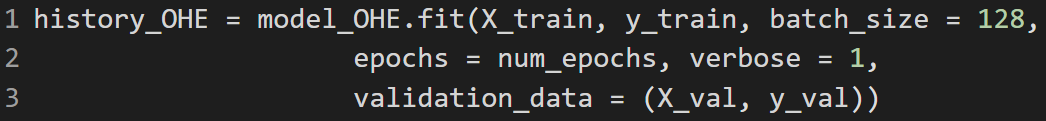
\includegraphics[scale=0.45]{Latex template for Project Report-20220108/immagini/ModelFit.png}
%      \caption{Codice metodo addestramento rete base}
%      \label{fig:modelFit}
% \end{figure}




\subsubsection{Dropout}
La prima tecnica considerata è \textit{Dropout}, metodo di regolarizzazione che permette durante la fase di training di considerare (in alcuni layer) solo una porzione casuale dei neuroni (e rispettive connessioni).
Il metodo che permette di definire la rete neurale base (\texttt{NeuralNetworkDropout()}) aggiungendo dei layer di Dropout dopo il secondo, terzo e quarto layer. Le percentuali di neuroni rimosse, selezionate dopo diversi tentativi, sono le seguenti: 30\% al secondo layer, 20\% al terzo e 10\% al quarto.

\subsubsection{L1 e L2}
Si testano le tecniche \textit{L1}, che usa come funzione di regolarizzazione la somma dei pesi e penalizza maggiormente i pesi più piccoli, e \textit{L2}, che usa la somma dei quadrati dei pesi e penalizza i pesi più grandi.
\texttt{NeuralNetworkL1\_L2()} ridefinisce la rete base aggiungendo la regolarizzazione \textit{L1} o \textit{L2}, determinata attraverso il parametro \texttt{l1} e applicata a ogni layer eccetto l'ultimo. Sia i kernel regularizers che i bias regularizers utilizzano uno stesso valore di regolarizzazione che però cambia tra \textit{L1} e \textit{L2} (rispettivamente 0.001 e 0.01), ed è stato scelto dopo una serie di sperimentazioni.

%I risultati ottenuti da \textit{L1} sono i seguenti: la validation riporta valori di \textit{accuracy} e di \textit{loss} peggiori rispetto a quelli del training set, portando quindi a ipotizzare una situazione di overfitting che abbiamo potuto riscontrare anche nei grafici, visibili nel \href{https://colab.research.google.com/drive/1SPoqJncv_oZZa3kvBMZnVyedcMGaKDti?usp=sharing}{notebook}, in cui la loss del validation set però tende a crescere anziché diminuire. L'accuracy invece si stabilizza su un valore non alto e smette presto di crescere. 

%I risultati ottenuti da \textit{L2} sono i seguenti: la validation riporta valori di \textit{accuracy} e di \textit{loss} peggiori rispetto a quelli del training set, portando quindi a ipotizzare una situazione di overfitting che abbiamo potuto riscontrare anche nei grafici, visibili nel \href{https://colab.research.google.com/drive/1SPoqJncv_oZZa3kvBMZnVyedcMGaKDti?usp=sharing}{notebook}, in cui la loss del validation set però tende a crescere e diminuire leggermente verso le ultime epoche. L'accuracy invece continua a crescere durante le epoche. 
%In generale i valori raggiunti con il validation set sono sufficienti ma non eccellenti in entrambi i modelli. Entrambe le tipologie di regolarizzazione vengono sperimentate su 300 epoche i cui risultati sono riportati nella tabella \ref{table:l1l2}.

\subsubsection{L2 e Dropout}
È stato poi effettuato un tentativo combinando le tecniche di \textit{L2} e \textit{Dropout}, tramite il metodo \texttt{NeuralNetworkL2\_drop()}, per cercare di ottenere risultati migliori. 
Infatti, dall'osservazione dell'andamento della history (Figura \ref{fig:primiModelli}) viene scelto di continuare le sperimentazioni utilizzando \textit{L2}, anziché \textit{L1}.
Per il \textit{Dropout} sono state scelte percentuali più basse in modo da non incidere troppo con la regolarizzazione sul modello. In particolare nel secondo, terzo e quarto strato viene rimosso il 10\% dei neuroni.

%Da cui possiamo notare essere molto simili a quelli precedentemente ottenuti con \textit{L2}, ma la \textit{loss} sul validation set risulta migliore rispetto a quella ottenuta con solo \textit{Dropout}.

\subsubsection{Early Stopping (ES)}
La quarta tecnica di regolarizzazione utilizzata è \textit{Early Stopping} \textit{(ES)} \cite{machinelearningmasteryEarlyStopping}, che consente di ritornare al miglior modello ottenuto durante la fase di training se esso non coincide con l'ultimo ottenuto.
Risulta quindi necessario definire la variabile \texttt{early\_stopping}, che specifica la variabile da monitorare durante il training, \texttt{validation loss}, e la \texttt{patience} da avere prima di decretare che il modello non stia migliorando. 
Dal momento che la loss ha un andamento molto oscillante (vedi Figura \ref{fig:secondiModelli}), è stata fissata una \texttt{patience} alta (70 epoche). Viene definito un \texttt{ModelCheckpoint} per salvare il miglior modello ottenuto nel training, scelto in base ai valori assunti da \textit{validation accuracy}. 
La tecnica \textit{ES} viene quindi aggiunta ai due migliori modelli ottenuti finora: \textit{L2} e \textit{L2} con \textit{Dropout}, vengono addestrate usando gli stessi parametri della rete base con l'aggiunta di \texttt{callbacks} per \textit{ES}.

%\href{https://colab.research.google.com/drive/1SPoqJncv_oZZa3kvBMZnVyedcMGaKDti?usp=sharing}{notebook}

%L'addestramento viene quindi bloccato alla 96esima epoca, la \textit{loss} calcolata sul validation set stava continuando a crescere. 

%Confrontando con i valori di \textit{accuracy} e \textit{loss} ottenuti (riportati nella tabella \ref{table:l2es}) con i valori ottenuto con il modello \textit{L2} senza \textit{Early Stopping} notiamo che i valori ottenuti con il train set sono leggermente peggiori ma comunque molto buoni, mentre la \textit{loss} ottenuta con il \textit{validation set} è migliorata e l'\textit{accuracy} ottenuta con il \textit{validation set} leggermente peggiorata.
%Nel complesso, non sembrano esserci sostanziali differenze tra i due modelli.


%L'addestramento viene bloccato alla 165esima epoca.

%La particolarità di questo addestramento è che neanche dai risultati ottenuti sul \textit{training set} (visibili nella tabella \ref{table:l2dropes}) notiamo particolari miglioramenti nel corso delle epoche.
%Confrontando con i valori di \textit{accuracy} e \textit{loss} ottenuti con il modello \textit{L2} e \textit{Dropout} senza \textit{Early Stopping} notiamo che i valori ottenuti con il train set sono ora leggermente migliori, mentre la \textit{loss} ottenuta con il \textit{validation set} è molto simile e l'\textit{accuracy} ottenuta con il \textit{validation set} è migliorata.
%Nel complesso, anche in questo caso le differenze sono minime. Confrontando invece con i risultati ottenuti con \textit{L2} e \textit{Early stopping} notiamo che per quanto riguarda la \textit{validation}, l'\textit{accuracy} è migliore con il \textit{Dropout}, mentre la \textit{loss} peggiore. 

\subsubsection{Class Weight (CW)}

Al fine di migliorare i risultati ottenuti e gestire lo sbilanciamento della variabile target, viene fatto un tentativo di \textit{Class Weighting (CW)} \cite{kerasKerasDocumentation}\cite{tensorflowClassificazioneDati}. Il metodo \texttt{compute\_class\_weight} di \textit{Keras}, che permette di assegnare un nuovo peso alle classi del target, in modo da bilanciare le loro occorrenze nel dataset: i pesi più alti vengono assegnati alle classi minoritarie.
\textit{CW} e \textit{ES} vengono quindi applicati ai due modelli \textit{L2} e \textit{L2-Dropout}, addestrandole usando gli stessi parametri
della rete base con l'aggiunta di \texttt{callbacks} e  \texttt{class\_weight}.

%\textit{Early Stopping} porta l'addestramento a interrompersi alla 72esima epoca.

%\href{https://colab.research.google.com/drive/1SPoqJncv_oZZa3kvBMZnVyedcMGaKDti?usp=sharing}{notebook}) possiamo notare una crescita della \textit{validation accuracy} e un'iniziale crescita, seguita da una decrescita della \textit{validation loss} (motivo per cui l'addestramento si interrompe dopo così poche epoche). 

%Confrontando con i valori di \textit{accuracy} e \textit{loss} ottenuti (riportati nella tabella \ref{table:l2dropes}) con il modello \textit{L2 Early Stopping} senza \textit{Class Weight}, notiamo che sul training set ora otteniamo valori migliori, mentre sul validation set la \textit{loss} è peggiorata mentre l'\textit{accuracy} e migliorata. 
%Come nei casi precedenti, i risultati dei due modelli confrontati non distano poi molto fra loro.

%\textit{Early Stopping} porta l'addestramento a interrompersi alla 74esima epoca.

%Entrambe \textit{loss} e \textit{accuracy} risultano essere oscillanti, come si può riportare dai grafici riportati nel e dai grafici (riportati nel nel \href{https://colab.research.google.com/drive/1SPoqJncv_oZZa3kvBMZnVyedcMGaKDti?usp=sharing}{notebook}), ma si può notare come la \textit{validation loss} in un primo momento cresce, per poi decrescere. Non sono comunque più stati raggiunti gli iniziali risultati, motivo per cui dopo 70 epoche di non miglioramento, l'addestramento è stato interrotto.

%Confrontando con i valori di \textit{accuracy} e \textit{loss} ottenuti, riportati nella tabella \ref{table:l2escw} con il modello con \textit{L2, Dropout e Early Stopping} ma senza \textit{Class Weight} notiamo che la \textit{training loss} è leggermente peggiorata, mentre la \textit{training accuracy} leggermente migliorata. 
%Stessa situazione riscontriamo anche per \textit{accuracy} e \textit{loss} del \textit{validation set}. 
%Le differenze risultano però essere minime.
%Confrontando invece con i risultati ottenuti con il modello con \textit{L2} e \textit{Early Stopping}, notiamo che per quanto riguarda il training, ora otteniamo risultati migliori, mentre per la \textit{validation} solo l'\textit{accuracy} è di poco migliore.